\documentclass[11pt]{article}
\usepackage{uspstyle,amssymb,graphicx,amsmath, caption, subcaption}

\graphicspath{ {./images/} }

\begin{document}

\maketitle

% The content of your research proposal, including text, figures and images, 
% should not exceed 5 pages, typed, double-spaced (additional pages may be 
% included for your works-cited/references).

\section{Introduction}
% Provide a statement of the objective(s) and the anticipated significance of the 
% work to your field of study. What problems will be investigated? What hypothesis 
% will be tested? We suggest that the introduction begin with a brief description 
% of the project in general terms before the more technical aspects of the project 
% are discussed. 

Computational topology can broadly be described as the extension of techniques
from the pure math field of topology to a discrete and algorithmic setting
widely applicable to point cloud data. Computational topology often deals with data
in the form of a simplicial complex, which may be arbitrarily high dimensional.
One of the major goals of computational topology is to describe these simplicial
complexes in terms of their connected components and their cycles in any dimension.
In practice, these features frequently describe important attributes of data, with
applications including mapping various networks, cancer screening,
encryption, quantum physics, machine learning, and neuroscience.

I too am interested in this problem of capturing topological features in data,
and am particularly captivated by a field known as discrete Morse theory.
Morse theory arises out of classical topology as a set of
methodologies to detect topological features by assigning a function to a topological
space. Discrete Morse theory (DMT) attempts to construct similar functions, but in a computational
setting. In other words, DMT seeks to generate topologically meaningful functions on a simplicial
complex. Work has been done to algorithmically generate discrete Morse functions on a simplicial complex, 
but this specific area of research is relatively new and remarkably limited. I plan to expand upon
the work that I, Brad McCoy, Dr. Brittany Fasy, and Dr. David Millman have conducted in the last year
to improve upon existing algorithms which construct discrete Morse functions on a simplicial complex.
In doing so, I aim to provide novel insights into how topological features may be detected in data.
Consequently, I hope to move forward the viability of discrete Morse theory as an approach to the 
wide array of applications of computational topology mentioned above.

\begin{figure}
\centering
\begin{subfigure}{.5\textwidth}
  \centering
	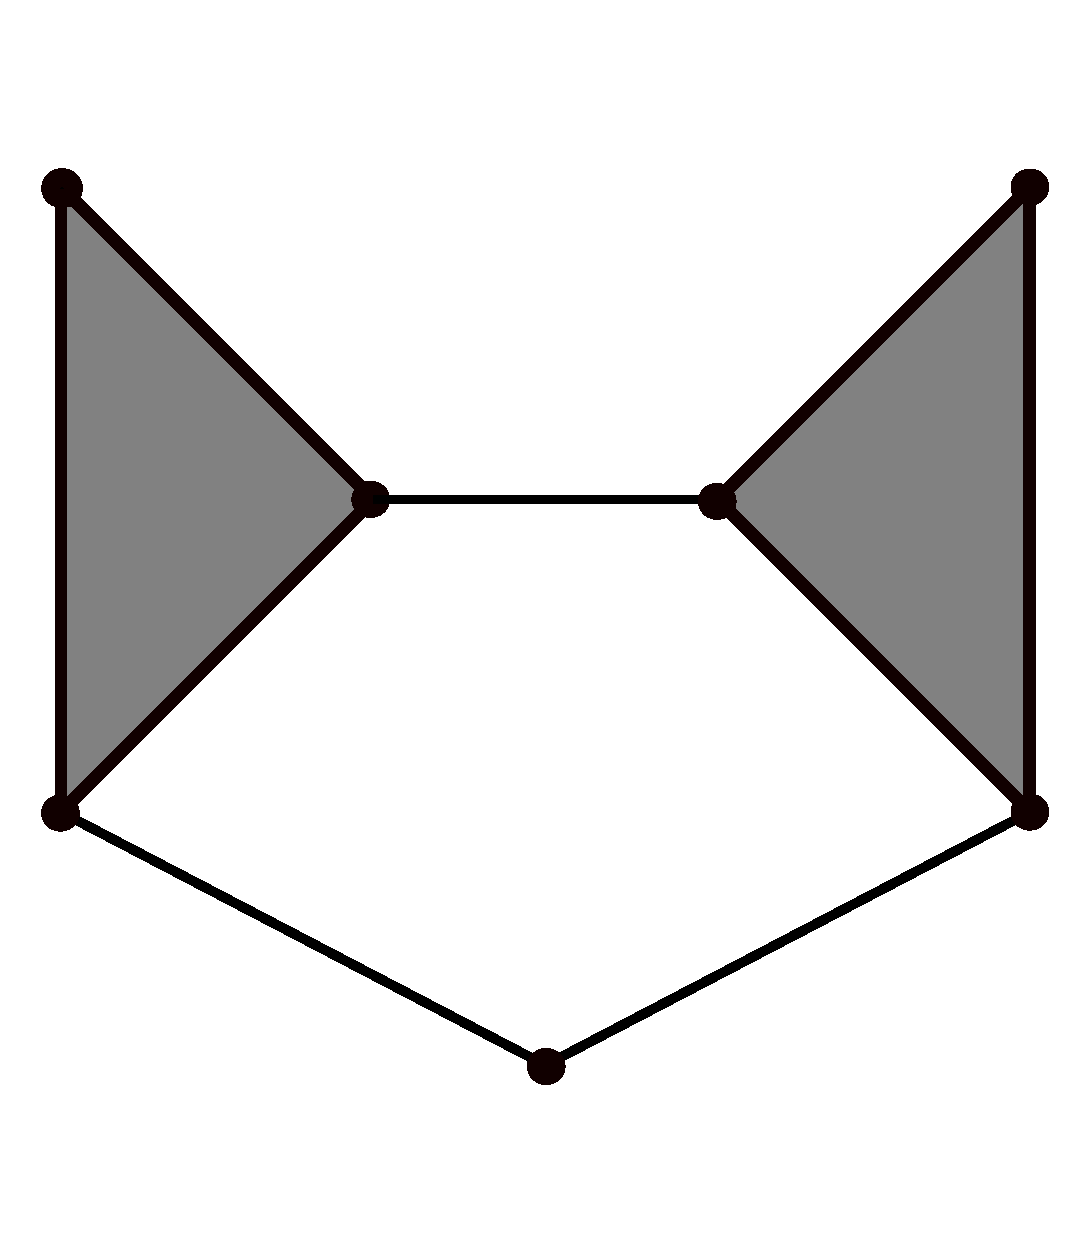
\includegraphics[width=.25\linewidth]{cat.pdf}
	
\includegraphics[width=.25\linewidth]{arrow.pdf}
	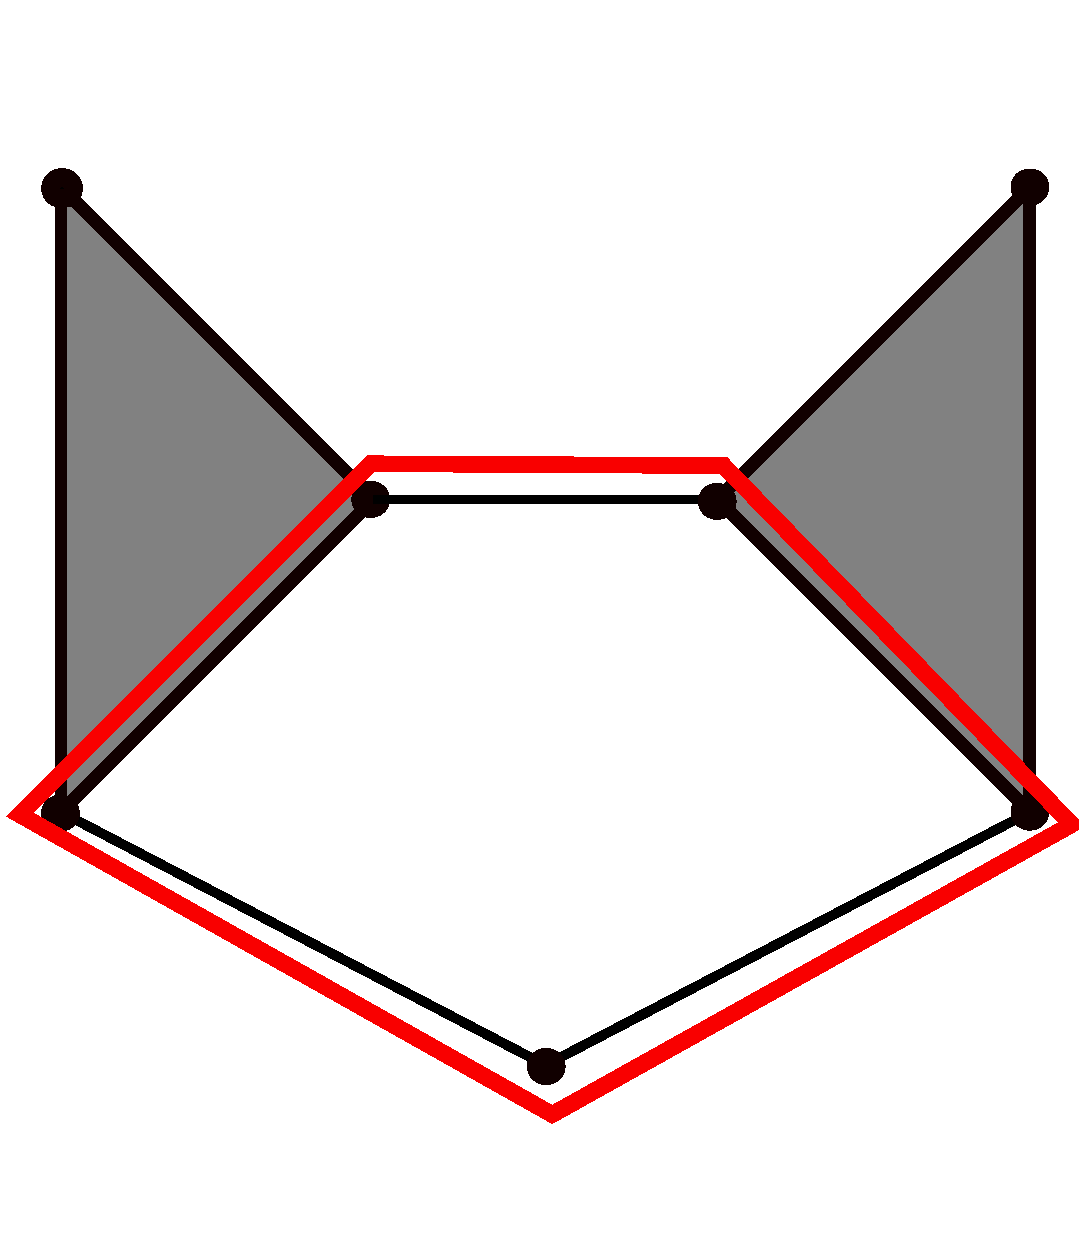
\includegraphics[width=.25\linewidth]{redcat.pdf}
	\caption{Example simplicial complex with red cycle.}
  \label{fig:sub1}
\end{subfigure}%
\begin{subfigure}{.5\textwidth}
  \centering
  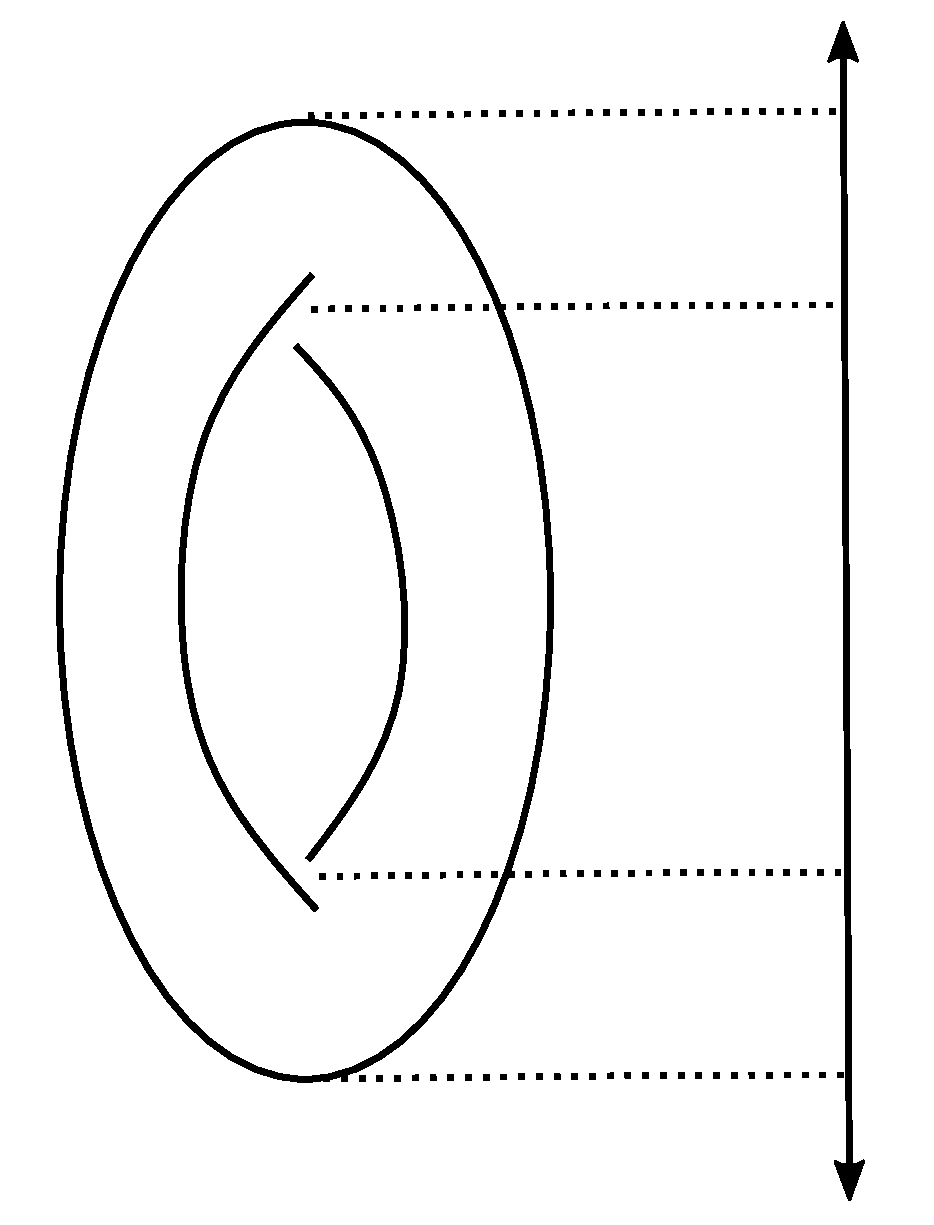
\includegraphics[width=.4\linewidth, height=3cm]{torus.pdf}
	\caption{An example smooth Morse function, whose critical points reveal topological features.}
  \label{fig:sub2}
\end{subfigure}
	\caption{We want to detect topological features in a simplicial complex (such as the cycle in red on the bobcat shaped complex), using functions similar to classical Morse theory height functions.}
\label{fig:test}
\end{figure}


\section{Background}
% Provide a brief review of the work that has been done in the project 
% area together with complete references in appropriate professional style. This 
% section should also include any personal information about you that would 
% indicate to the reviewers your qualifications for successfully completing this 
% project, including a statement of how the project will contribute to your 
% academic and career goals.

Milnor’s classical Morse theory provides tools for investigating 
the topology of smooth manifolds \cite{milnor63}. 
In \cite{forman98},
Forman showed that many of the tools for continuous
functions can be applied in the discrete setting. Inferences 
about the topology of a simplicial complex can be made
from the number of critical cells in a Morse function on
the complex.
Given a Morse function one can interpret the function 
in many ways. Switching interpretations is often
revealing. In previous work, we've found it particularly useful
to think of a discrete Morse
function in three different ways. Algebraically, a Morse
function is a function from the faces of a complex to the
real numbers, subject to certain inequalities. Topologically, 
a Morse function is a pairing of the faces such that
the removal of any pair does not change the topology of
the complex. Combinatorially, a Morse function is an
acyclic matching in the Hasse diagram of the complex,
where unmatched faces correspond to critical cells.

In \cite{us}, we provided a new algorithm we call \textsc{ExtractRightChild} to compute
a rudimentary discrete Morse function on a simplicial
complex which improved the time complexity of pre-existing
algorithms. To do so, we primarily focused on generating
discrete Morse functions in a combinatorial setting,
via matchings in the Hasse diagram. We were pleased with our result,
which builds on algorithms proposed in \cite{king},
but our algorithm can be refined. In particular, 
\textsc{ExtractRightChild} may output a large number of critical
cells, which means that there may exist possible Morse functions
which are more strongly indicative of the topology of a complex.
This is the main area of work for the upcoming year- to 
propose efficient new algorithms which further refine the output of 
\textsc{ExtractRightChild}. Along with this, a major area of
research is also to bound the number of critical cells produced
by \textsc{ExtractRightChild}. In each of these research objectives, 
we aim to propose increasingly
reliable indicators of the topology of a simplicial complex, which may 
pose wider implications throughout the field of computational topology in the 
future.

Discrete Morse theory has been particularly effective when combined with persistent 
homology to analyze data, as is done in
\cite{king,uli-phd,bauer2012optimal,edelsbrunner02,wang18,vcomic2011dimension,edelsbrunner2003hierarchical}.
This is also an active avenue of research, to tie discrete Morse theory to
exciting new applications in persistent homology.
When dealing with data, we so far worked with the 
additional constraint 
that vertices have function values assigned. For
complexes without any preassigned function values,
Joswig and Pfetsch showed that finding a Morse function 
with a minimum number of critical cells is NP-Hard
\cite{joswig04}. Algorithms that find Morse functions with relatively 
few critical cells have been explored in 
\cite{lewiner03,nanda2013morse,hersh05}.
This presents yet another area to pursue in the upcoming year,
which is to construct Morse functions on data with more sparsely 
pre-assigned function values, like for instance on higher dimensional simplices.
Furthermore, all of our recent results have been purely theoretical,
and their implementation in a programming setting
would undoubtedly be of use in the future and is another focus of the project.

\begin{figure}
\centering
	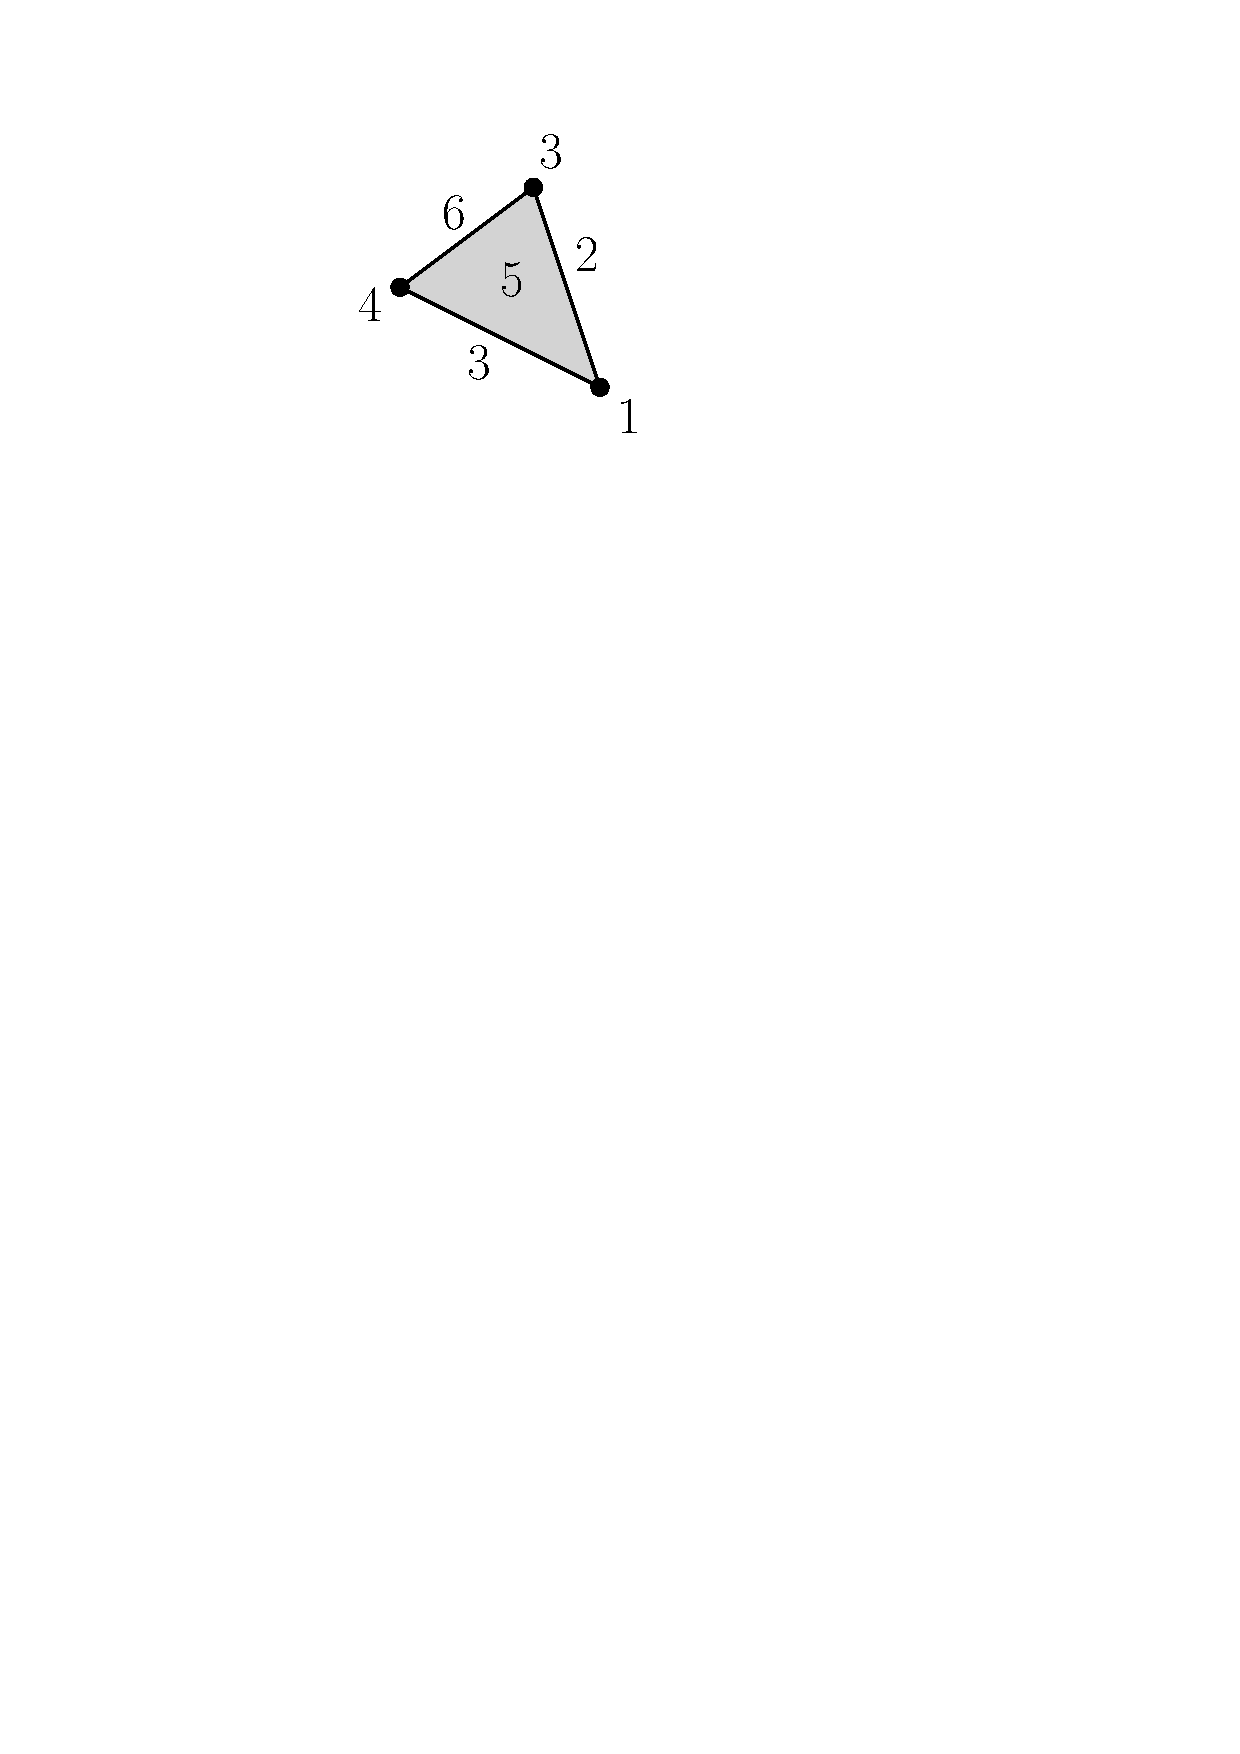
\includegraphics[scale=0.65]{algebra.pdf}
	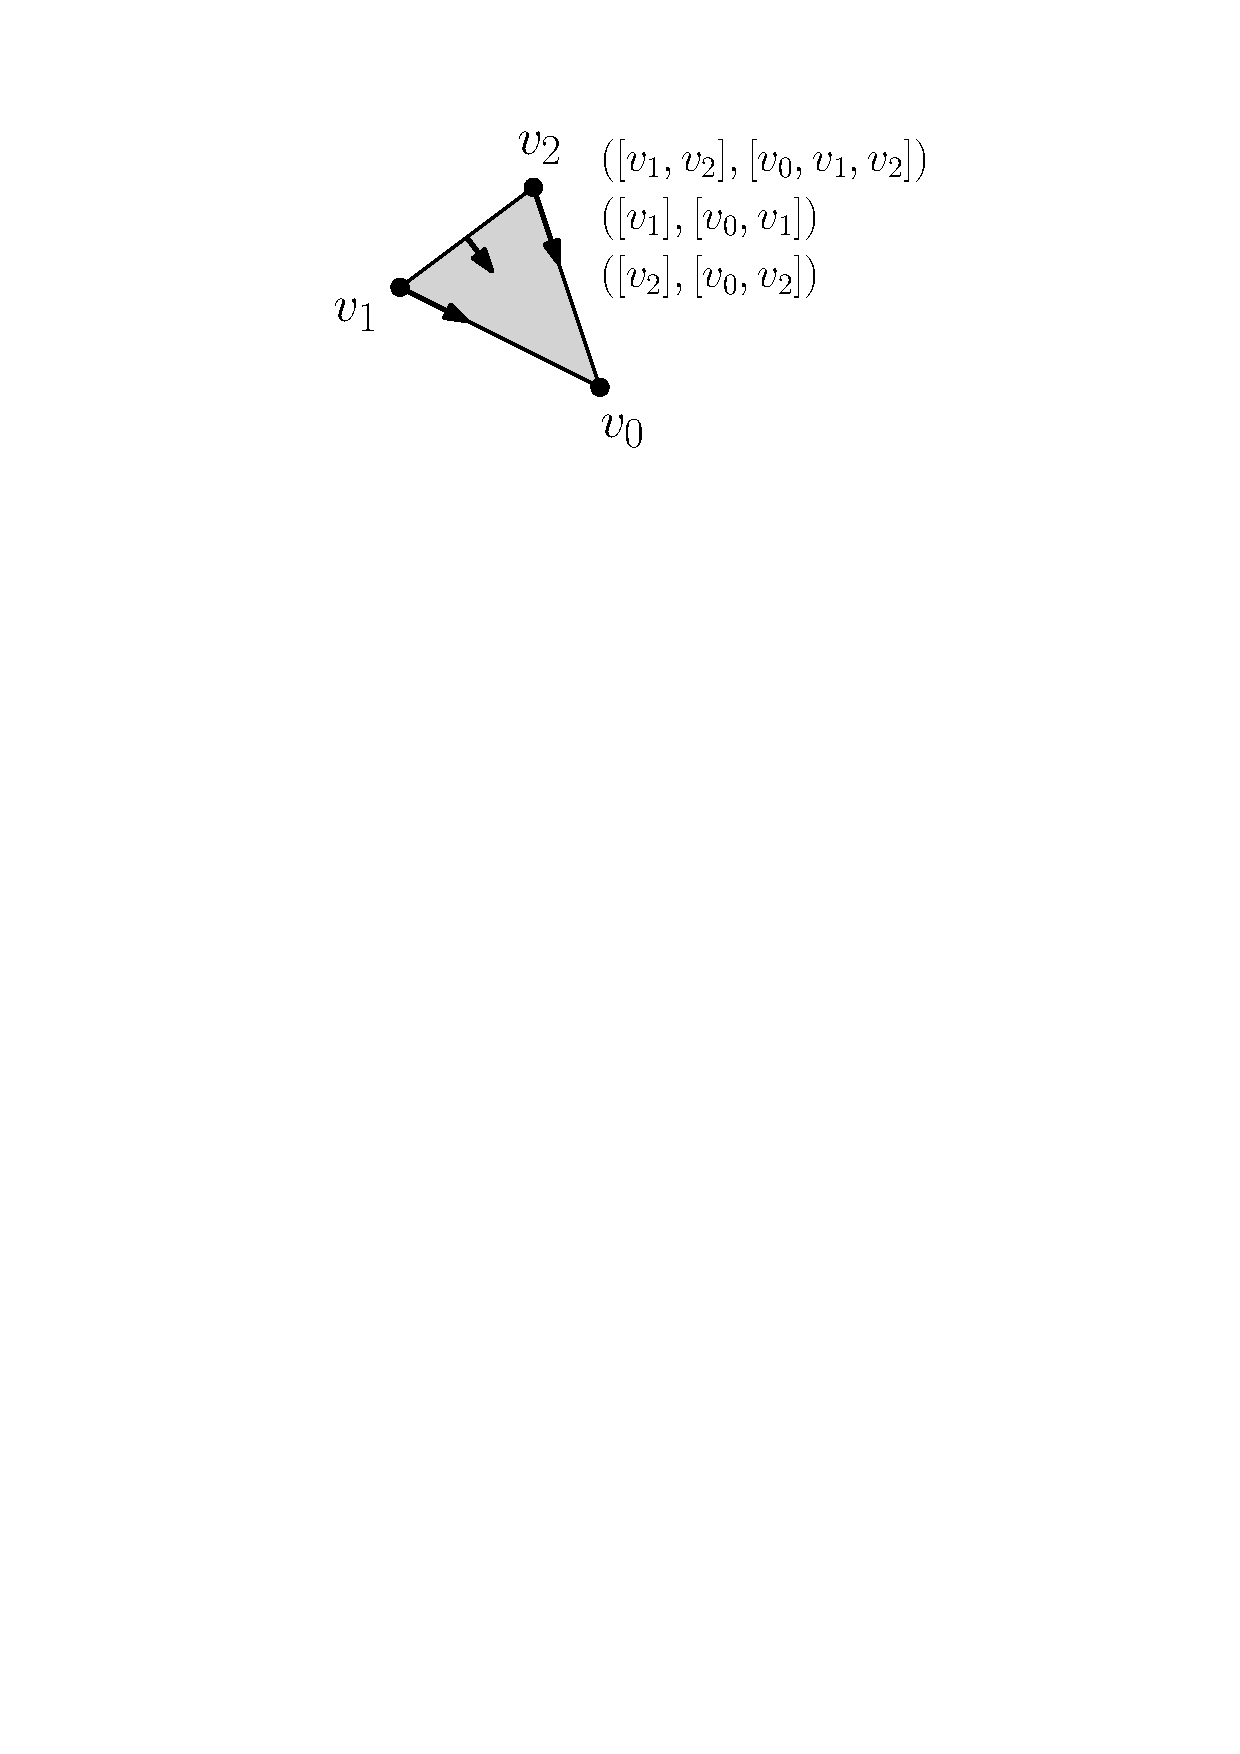
\includegraphics[scale=0.65]{topology.pdf}
	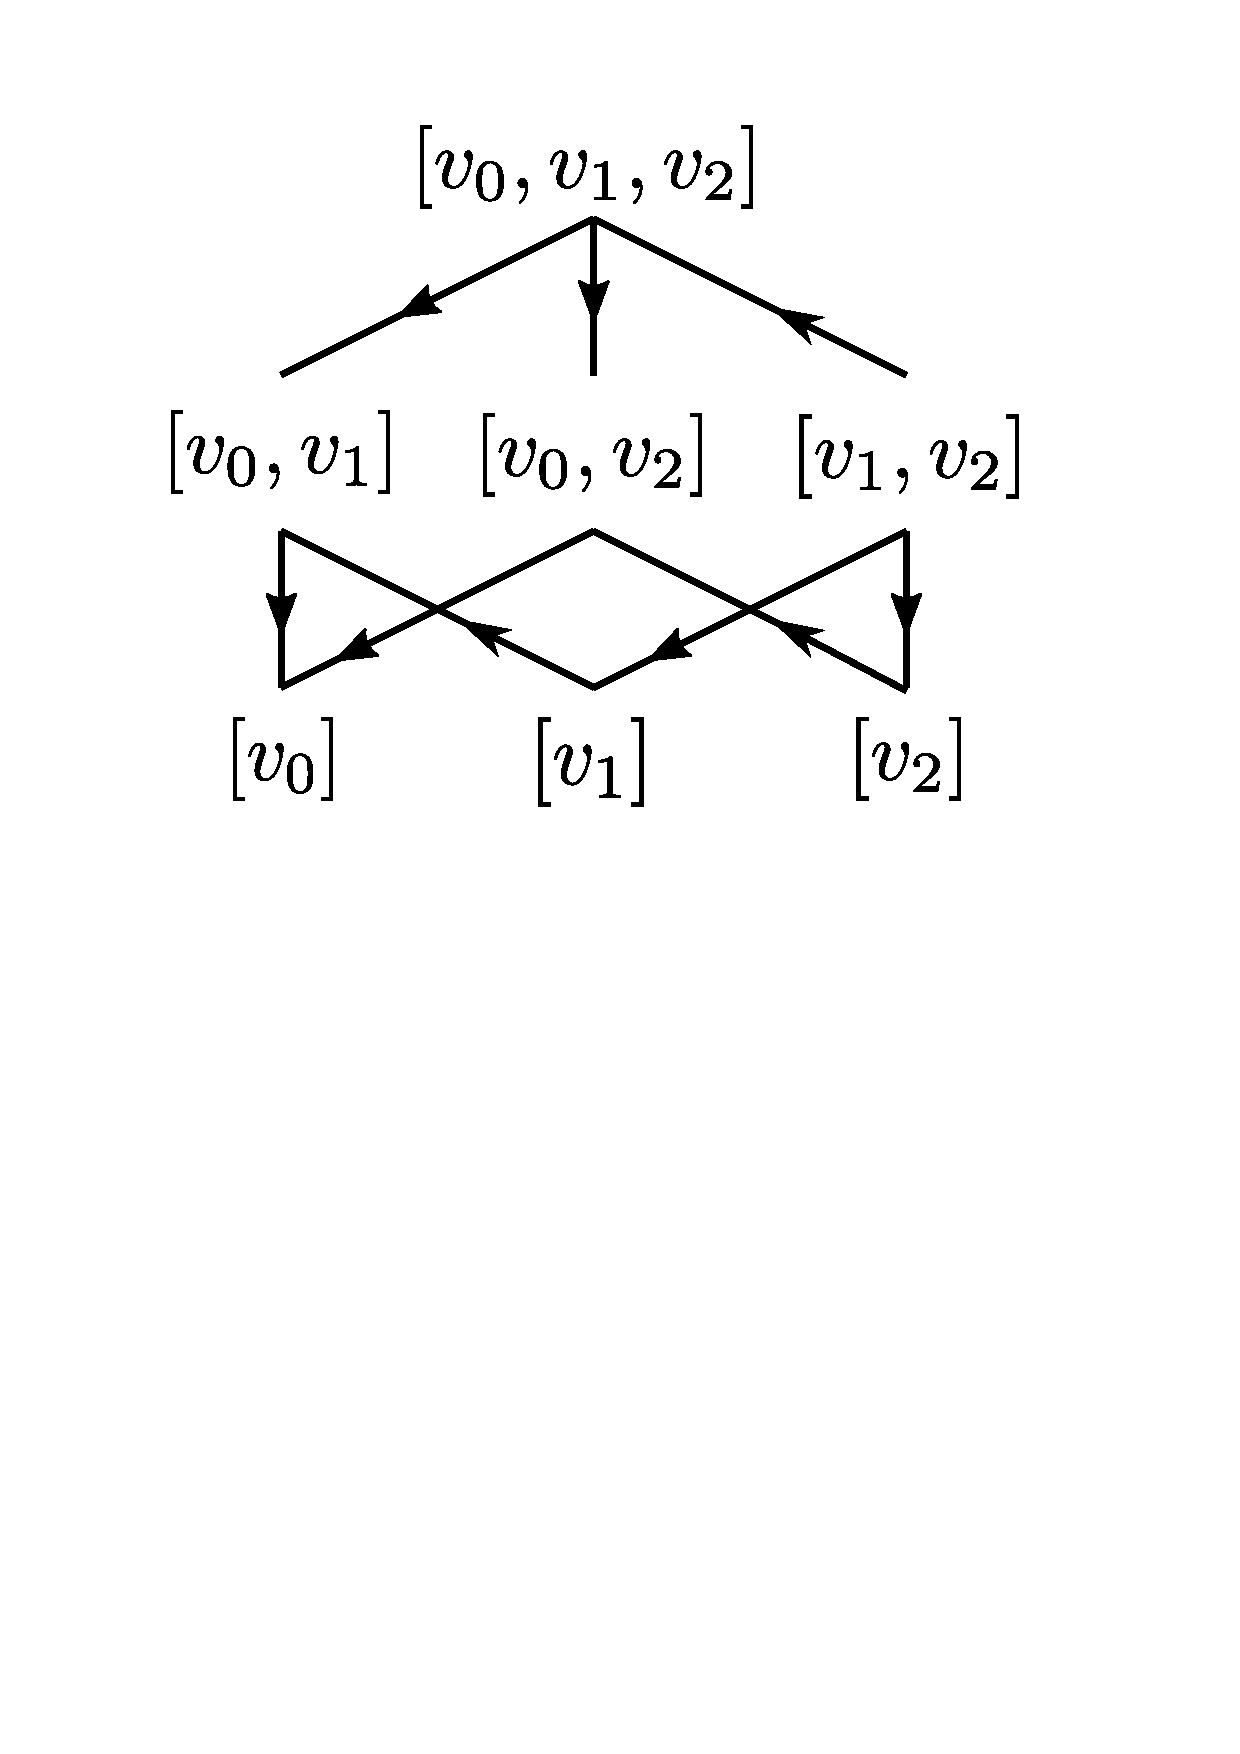
\includegraphics[scale=0.25]{combinatorics.pdf}
	\caption{The three mathematically equivalent ``flavors" of discrete Morse functions we're concerned with. From left to right, these are algebraic, topological, and combinatorial.}
\end{figure}


\begin{figure}
\centering
\begin{subfigure}{.33\textwidth}
  \centering
  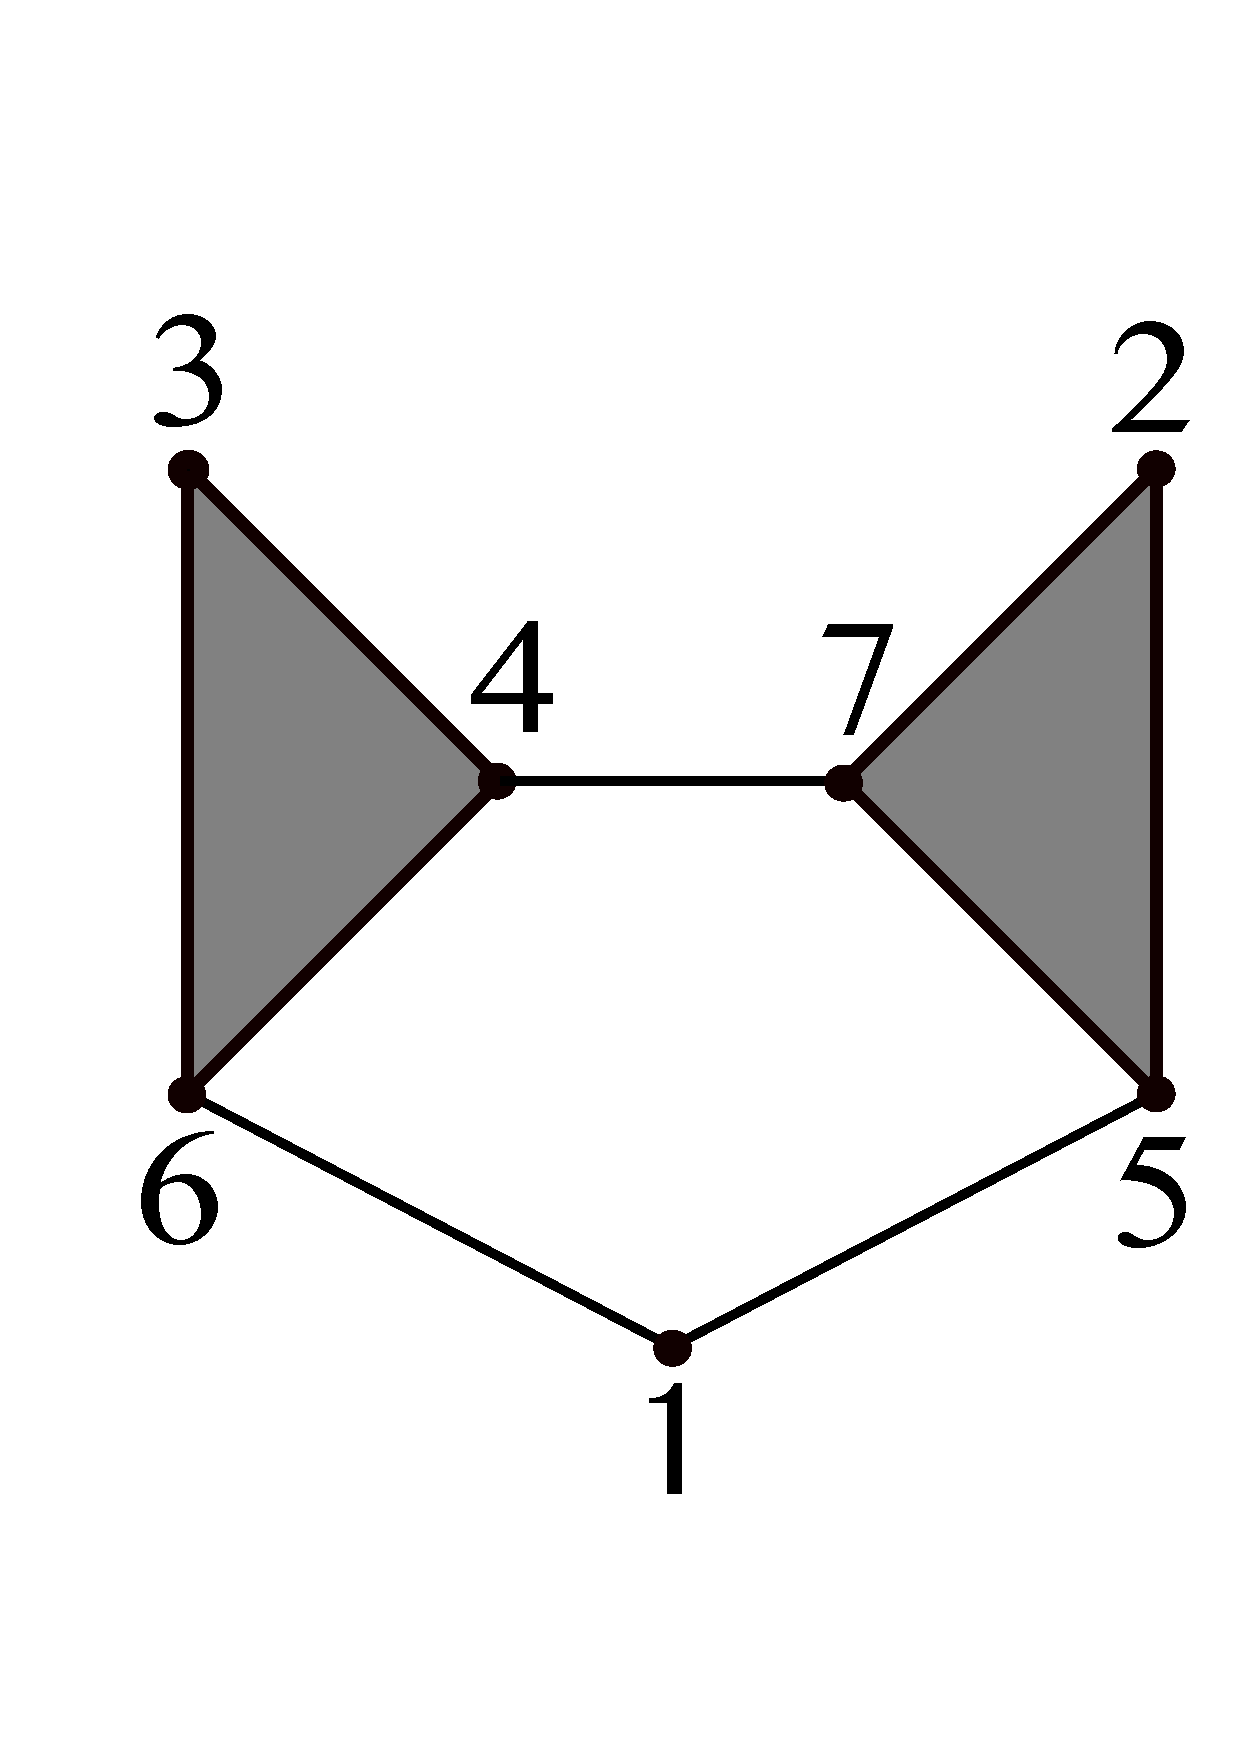
\includegraphics[width=.4\linewidth]{cat2.pdf}
  \caption{Bobcat simplicial complex with pre-existing data on the vertices}
  \label{fig:sub1}
\end{subfigure}%
\begin{subfigure}{.33\textwidth}
  \centering
  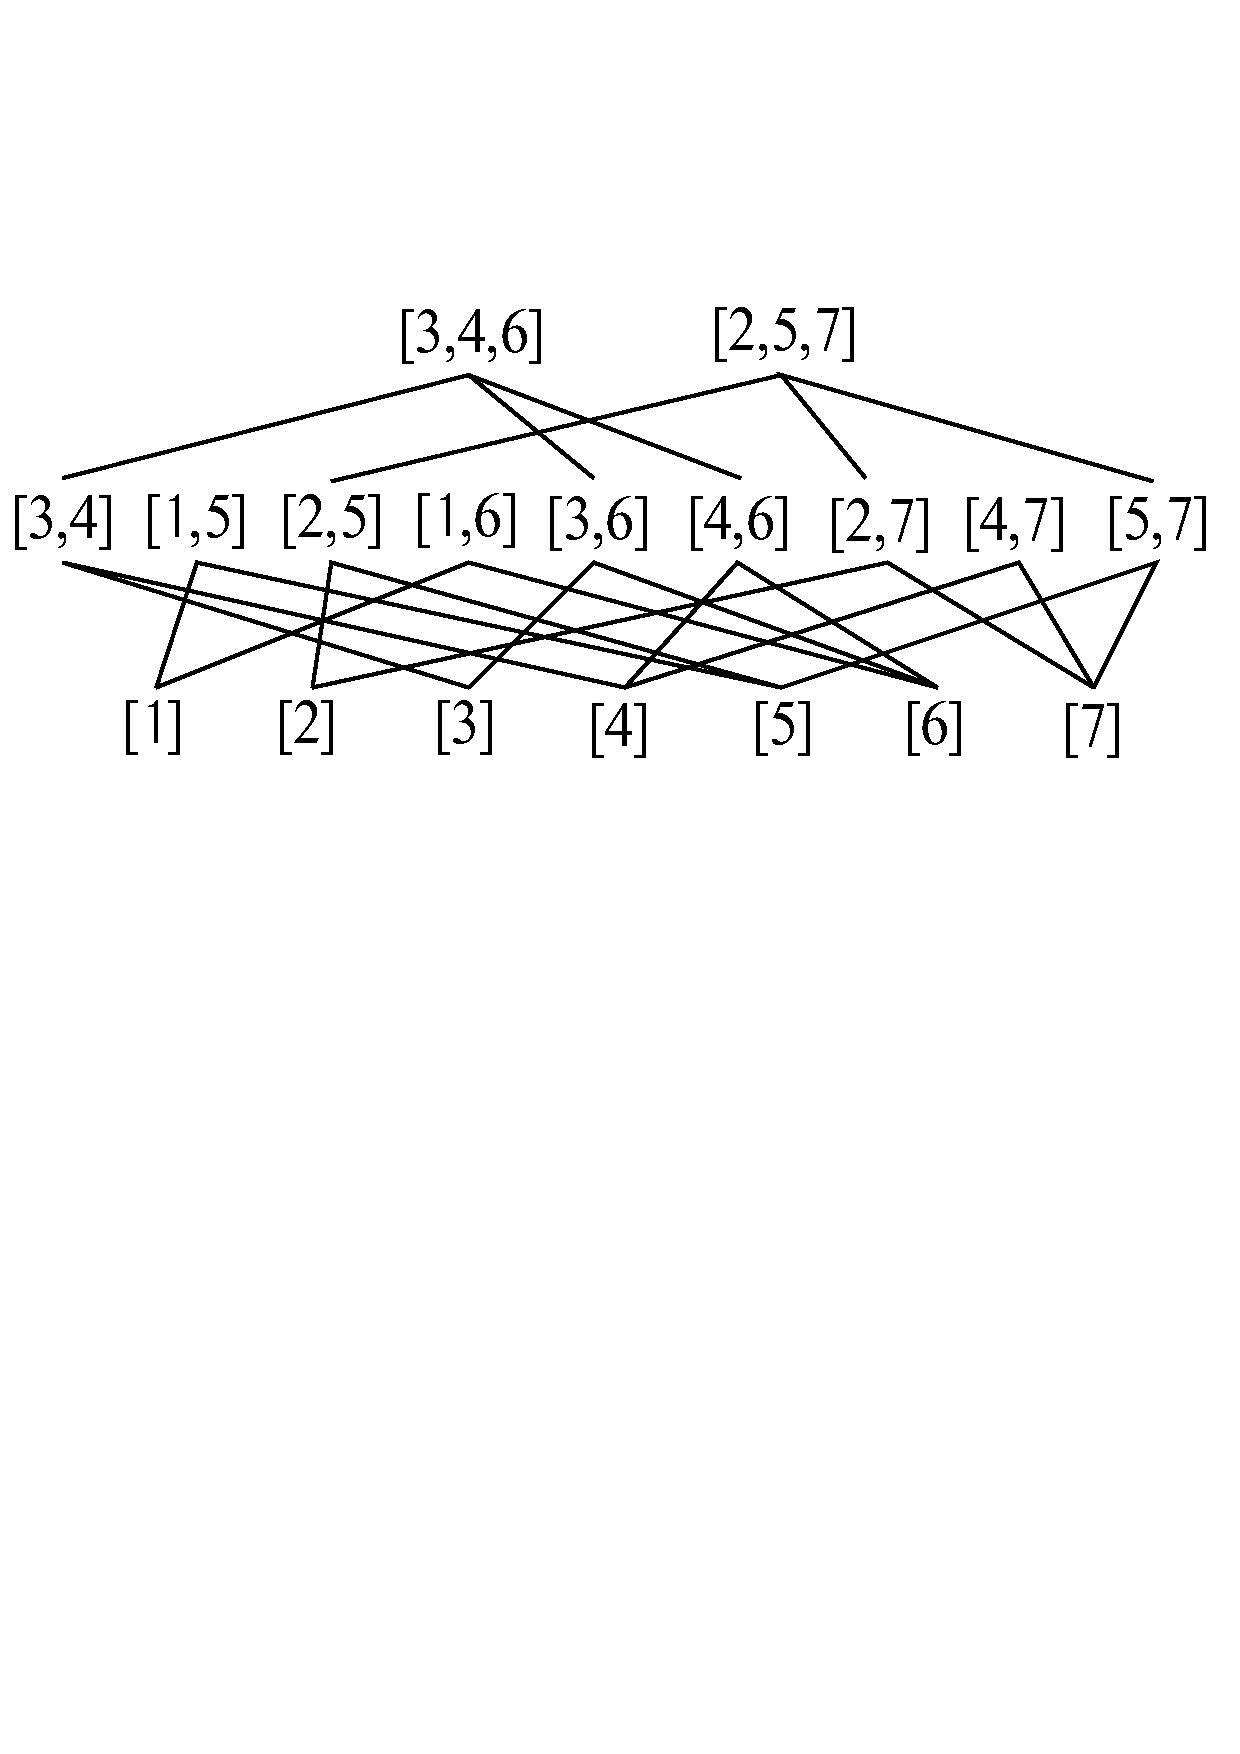
\includegraphics[width=.95\linewidth]{cat-hasse-sorted.pdf}
  \caption{Equivalent Hasse diagram}
  \label{fig:sub2}
\end{subfigure}
\begin{subfigure}{.33\textwidth}
  \centering
  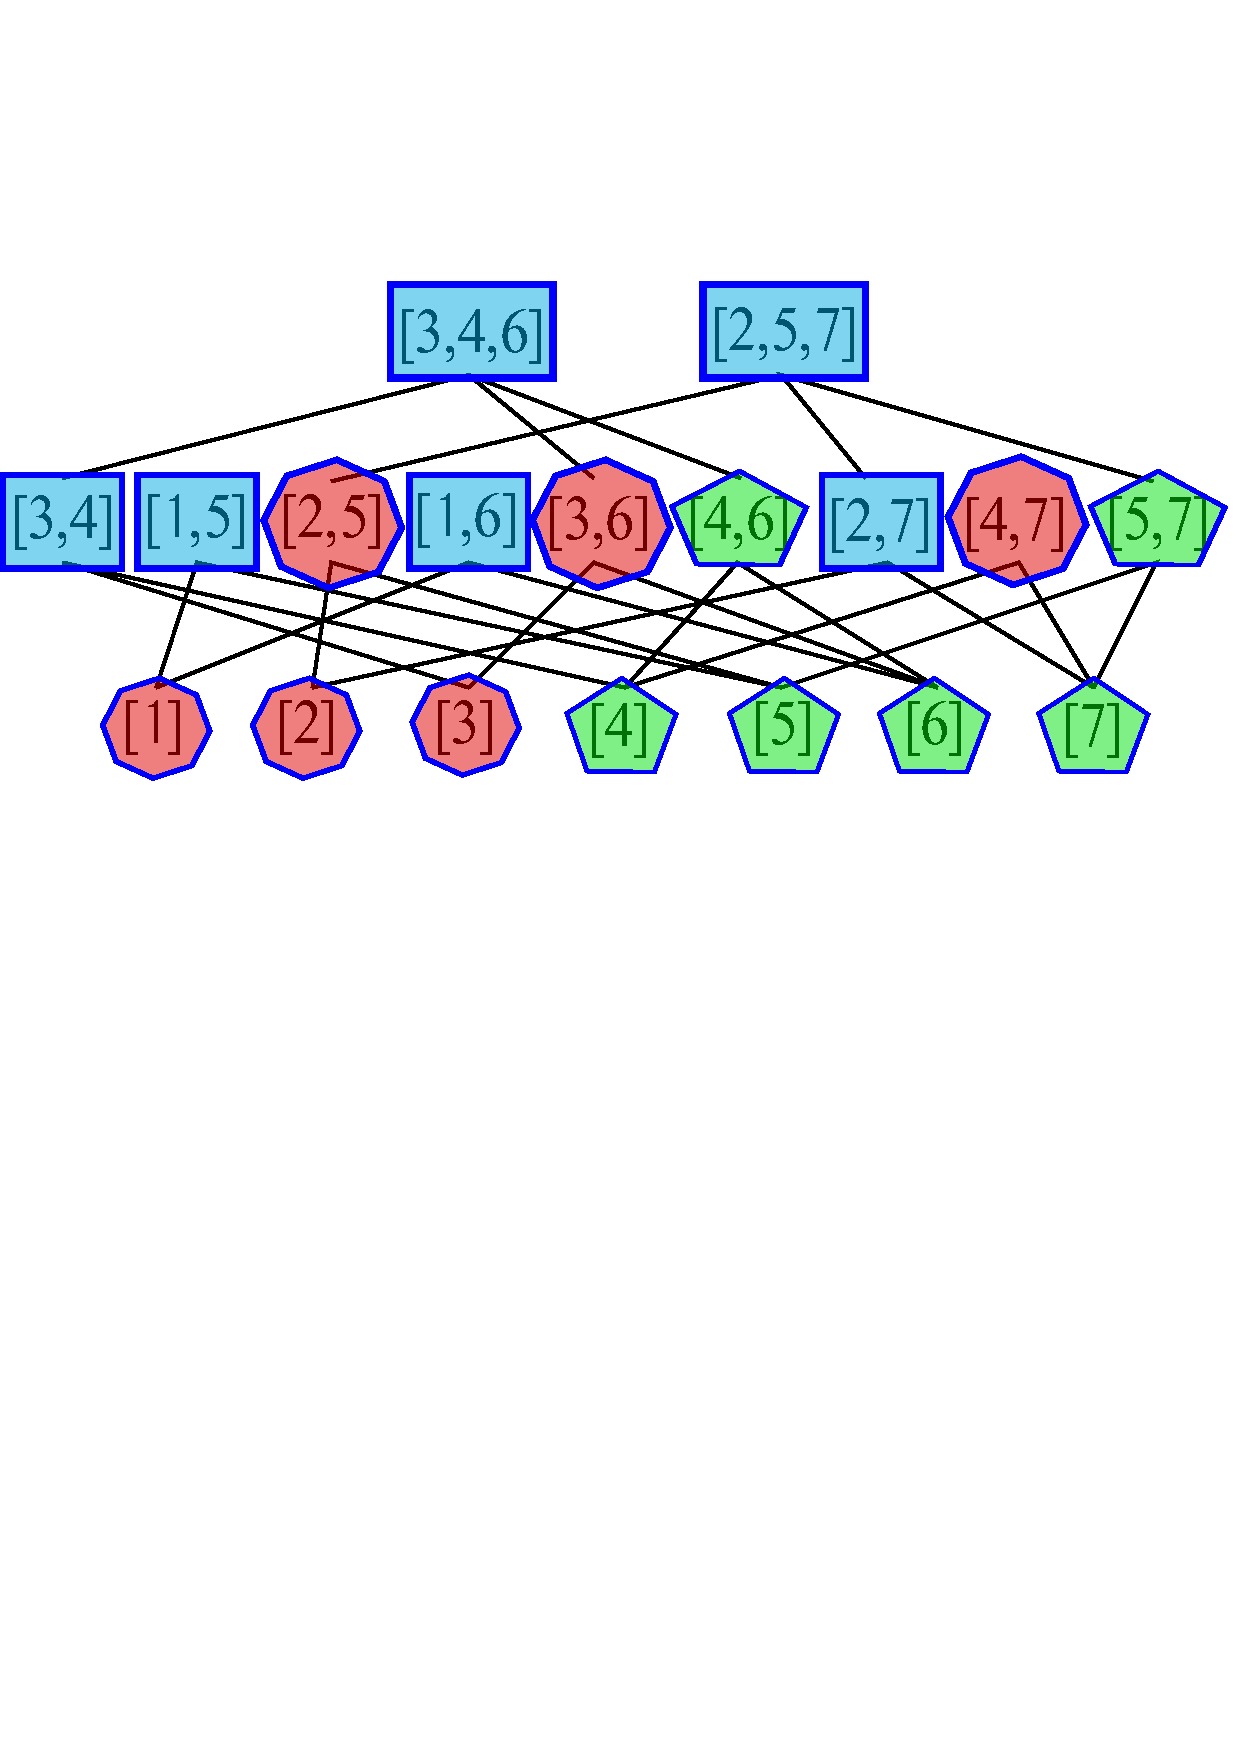
\includegraphics[width=.95\linewidth]{cat-alg5.pdf}
	\caption{Sample output of \textsc{ExtractRightChild}}
  \label{fig:sub3}
\end{subfigure}
	\caption{An example run of \textsc{ExtractRightChild}, where output matchings are shown by the heads of arrows in blue, the tails of arrows in green, and critical cells in red. This is a case where we have more critical cells than are exactly indicative of the topology. (One critical vertex and one critical edge would be the optimal output for this example.)}
\label{fig:test}
\end{figure}

\section{Methods}
% Provide a detailed description of the research methods that you will 
% use in the project. This should include a justification for the specific 
% approach that you will use. For example, how do the methods answer the questions 
% that have been posed, test the hypothesis, or lead to the desired goal?
% Timeline: Provide dates for the initiation and completion of each phase of the 
% project. Attempt to lay out a reasonable schedule taking into consideration all 
% phases of the research and final deliverables.
In order to successfully build upon the previous work I've conducted with other members
of the compTAG group at MSU, I plan to continue working as collaboratively with my
groupmates as possible, despite being in the midst of a pandemic. Over the past few months,
work on these types of problems has been accomplished using collaborative
whiteboard tools in a remote setting. Our group seems to have settled on using Miro,
an online whiteboard environment, which has helped us to regain the levels of productivity
we've had in person in previous years. More specifically, we will continue weekly hour long
group meetings where I will meet on Miro with Brad McCoy (a PhD student), Dr. Brittany Fasy,
and Dr. David Millman (my research advisors). In these meetings, we start by sharing recent 
developments and proofs we've written in the last week, then we often work together to iron out
our most recent results and to brainstorm next steps, and then establish our goals for the
upcoming week. These weekly meetings have been quite effective thus far, and I expect us to
continue efficiently producing new results in this adjusted online format. Then throughout the
week, if any one of us is working on a particular proof and would like to collaborate, we use
Slack for group messaging, and often will get back into Miro to work out proofs together.
Furthermore, our entire compTAG group participates in weekly seminars, which discuss group
developments and new areas of research. These meetings, which are anticipated to happen via
Zoom for the academic year, are also an effective venue to learn and share results.

As for the specific outline of the project, the focus generally will be to create an algorithm
which refines the output of \textsc{ExtractRightChild}, attempt to bound its output, implement our algorithms,
and then formally write up our results for a conference in the spring (we will most likely try to be published 
again in the Canadian Conference on Computational Geometry). Along with this, throughout the process,
we will be open minded towards new, exciting applications of discrete Morse theory, particularly in the
realm of persistent homology. A slightly more rigorous schedule is as follows:

\begin{enumerate}
	\item Create a refining algorithm for \textsc{extractrightchild} with time complexity improvements on prior algorithms: 10 weeks
	\item Formally prove performance of new algorithm in relation to pre-existing algorithms: 4 weeks
	\item Formally bound the number of critical cells produced by our new algoritm: 8 weeks
	\item Implement our algorithm: 2 weeks
	\item Formally write up and submit our results to a computational geometry conference: 4 weeks
\end{enumerate}

Due to the highly flexible nature of the research I'm conducting, this schedule is certainly subject to change.
However, based on prior results of a similar nature that my collaborators and I have generated, all of these 
tasks should be within reason to be accomplished roughly in the above timeframe. Along with this, due to the 
uncertainty of the world that we live in, research of this nature which is independent of physical experimentation or on-campus facilities seems to be a relatively reliable academic pursuit.

\section{Collaboration with Faculty Sponsor}
% Provide a description of the way you and 
% your faculty sponsor will collaborate on the project. The faculty sponsor should 
% play a significant role in responding to your ideas, providing advice for new 
% directions and resources, discussing the implications of the results, and 
% helping you prepare for your public presentation. Will there be regularly 
% scheduled meetings between you and your sponsor? Explain how the project relates 
% to the ongoing work of your sponsor, if this is the case.

As mentioned briefly above, the methodologies associated with this kind of theoretical 
research lend themselves well to collaboration with my research advisors. We will continue
our weekly meetings for the duration of the year, and I will also be an active member of 
our group's weekly seminars. This project ties in closely with the work of both of my advisors,
as discrete Morse theory is an increasingly influential field in computational topology.
Both of my mentors do a great deal of research in persistent homology, where these results
will be directly applicable. I have no doubt that with the guidance of my mentors this will be
another excellent and productive year of research. They have already equipped me well in the past
not only with the tools to effectively produce theoretical results, but also to have successful
experiences in the context of gaining publications and participating in conferences in the field.
I am incredibly excited to see what we are able to accomplish in another year of collaboration.

% Please draft your proposal in a format that is appropriate for your academic 
% discipline (i.e. MLA, APA, etc.) - consult your mentor if you have questions 
% about what format is most appropriate to your field of study
%%%%%%%%%%%%%%%%%%%%%%%%%%%%%%%%%%%%%%%%%%%%
%% BIBLIOGRAPHY
 \newpage
 \bibliographystyle{acm}
 \bibliography{references}
%%%%%%%%%%%%%%%%%%%%%%%%%%%%%%%%%%%%%%%%%%%%
% References Cited (include in an additional page within the project proposal): 
% Include a list of any literature that you have cited in the proposal. Nearly 
% all 
% good science and engineering proposals cite papers reporting related results, 
% describing the methods to be used or providing background information. Please 
% note-the review panel rarely recommends funding for proposals without adequate
% references.



\end{document}
